\documentclass{article}
\usepackage[utf8]{inputenc}
\usepackage{siunitx}
\usepackage[american,siunitx]{circuitikz}
\usepackage{amsmath}
\usepackage{svg}
\usepackage{booktabs}
\usepackage{float}
\renewcommand{\thesubsection}{\thesection.\alph{subsection}}
\newcommand{\equal}{=}

\title{ECE1101L\\Lab 10\\Voltage and Current Division}
\author{Choi Tim Antony Yung}
\date{7 November 2019}

\begin{document}

\maketitle

\section*{Objective}
The objective of this lab is to explore the voltage of individual resistors in a resistors circuit.

\section*{Lab Partner}
Antony Nursalim

\pagebreak

%1
\section{A circuit as illustrated below was set up with a \SI{6.00}{\volt} voltage source}
\begin{center}
    \begin{circuitikz}
        \draw 
            (1,2) 
            to[V_=$V_s\equal\SI{6}{\volt}$] (1,0)
            %(0,2) to[short,i>^=I] 
            %(1,2) to[R=\SI{1}{\kilo\ohm}] (3,2)
            (1,2)
            %--(3,2)
            to[R,l_=\SI{2}{\kilo\ohm} , v^=$V_1$] (5,2) --
            (6,2)to[R,l_=\SI{4.7}{\kilo\ohm} , v^=$V_2$] (6,0)--(1,0)
            ;
    \end{circuitikz}
\end{center}

%1a
\subsection{The resistance of the three resistors in circuit were measured}
The \SI{2}{\kilo\ohm} resistor was measured to have a resistance of \SI{1.983}{\kilo\ohm}, and the \SI{4.7}{\kilo\ohm} resistor was measured to have a resistance of \SI{4.680}{\kilo\ohm}.
\begin{table}[H]
\centering
    \begin{tabular}{@{}r r r r@{}}
         \toprule
         &measured & nominal & \%diff  \\
         \midrule
        $R_1$&\SI{1983}{\ohm} & \SI{2000}{\ohm} & -0.85\% \\
        $R_2$&\SI{4680}{\ohm} & \SI{4700}{\ohm} & -0.43\% \\ 
         \bottomrule
    \end{tabular}
\end{table}

%1b
\subsection{The voltage $V_1$ and $V_2$ can be calculated as follow}
\begin{align}
    \intertext{From voltage divider rule:}
    V_1 &= \frac{R_1}{R_t} \cdot V_s\\
    V_2 &= \frac{R_2}{R_t} \cdot V_s\\
    \intertext{Since the resistors are in series:}
    R_t &= \SI{1983}{\ohm} + \SI{4680}{\ohm} =\SI{6663}{\ohm}\\
    \intertext{Substituting $R_1 = \SI{1983}{\ohm}$, $R_2 = \SI{4680}{\ohm}$, $V_s = \SI{6.00}{\volt}$ and (3) into (1) and (2):}
    V_2 &= \frac{1983}{6663} \cdot \SI{6.00}{\volt} = \SI{1.786}{\volt}\\
    V_2 &= \frac{4680}{6663} \cdot \SI{6.00}{\volt} = \SI{4.214}{\volt}
\end{align}

%1c
\subsection{Voltage $V_1$ and $V_2$ was measured}
$V_1$ was measured to be \SI{1.787}{\volt} while $V_2$ was measured to be \SI{4.20}{\volt}

%1d
\subsection{The measured value of $V_1$ is slightly higher than the value calculated and the measured value of $V_2$ is slightly lower than the value calculated}
\begin{table}[H]
\centering
    \begin{tabular}{@{} l r r r@{}}
        \toprule
        &measured & calculated & \%diff  \\
        \midrule
        $V_1$ &\SI{1.787}{\volt} & \SI{1.786}{\volt} & 0.07\% \\
        $V_2$ &\SI{4.20}{\volt} & \SI{4.214}{\volt} & -0.34\% \\
        \bottomrule
    \end{tabular}
\end{table}

\pagebreak

%2
\section{A circuit as illustrated below was set up with a \SI{10.00}{\volt} voltage source}
\begin{center}
    \begin{circuitikz}
        \draw 
            (2,2) 
            to[V_=$V_s\equal\SI{10}{\volt}$] (2,-1)
            (2,2) --
            (3,2)to[R=$R_0\equal\SI{4.7}{\kilo\ohm}$] 
            (5,2)to[short,i=I]
            (6,2)to[short,i=$I_1$]
            (6,1)to[R,l_=$R_1\equal\SI{2}{\kilo\ohm}$] (6,-1)
            (6,2) -- 
            (9,2)to[short,i=$I_2$]
            (9,1)to[R,l_=$R_2\equal\SI{4.7}{\kilo\ohm}$] (9,-1)--(2,-1)
            ;
    \end{circuitikz}
\end{center}

%2a
\subsection{The resistance of the three resistors in circuit were measured}
The \SI{4.7}{\kilo\ohm} resistor was measured to have a resistance of \SI{4.670}{\kilo\ohm}, the \SI{2}{\kilo\ohm} resistor was measured to have a resistance of \SI{1.988}{\kilo\ohm}, and the second \SI{4.7}{\kilo\ohm} resistor was measured to have a resistance of \SI{4.680}{\kilo\ohm}.
\begin{table}[H]
\centering
    \begin{tabular}{@{}r r r r@{}}
         \toprule
         &measured & nominal & \%diff  \\
         \midrule
        $R_0$&\SI{4670}{\ohm} & \SI{4700}{\ohm} & -0.64\% \\
        $R_1$&\SI{1988}{\ohm} & \SI{2000}{\ohm} & -0.60\% \\ 
        $R_2$&\SI{4680}{\ohm} & \SI{4700}{\ohm} & -0.43\% \\
         \bottomrule
    \end{tabular}
\end{table}

%2b
\subsection{The current I was measured to be $\SI{0.001616}{\ampere}=\SI{1.616}{\milli\ampere}$}

%2c
\subsection{The current $I_1$ and $I_2$ can be calculated as follow}
\begin{align}
    \intertext{From current divider rule:}
    I_1 &= \frac{R_t}{R_1} \cdot I\\
    I_2 &= \frac{R_t}{R_2} \cdot I\\
    \intertext{The equivalent resistance of the resistors circuit can be calculated as follow:}
    R_t &= \SI{4670}{\ohm}+\frac{1}{\frac{1}{\SI{1988}{\ohm}} + \frac{1}{\SI{4680}{\ohm}}} =\SI{6065}{\ohm}\\
    \intertext{Substituting $R_1=\SI{1988}{\ohm}$, $R_2 = \SI{4680}{\ohm}$, $I=\SI{1.616}{\milli\ampere}$ and (8) into (6) and (7):}
    I_1 &= \frac{\SI{6065}{\ohm}}{\SI{1988}{\ohm}} \cdot \SI{1.616}{\milli\ampere}=\SI{1.134}{\milli\ampere}\\
    I_2 &= \frac{\SI{6065}{\ohm}}{\SI{4680}{\ohm}} \cdot \SI{1.616}{\milli\ampere}=\SI{0.482}{\milli\ampere}\\
\end{align}

%2d
\subsection{Current $I_1$ and $I_2$ was measured}
$I_1$ was measured to be \SI{1.127}{\milli\ampere} while $I_2$ was measured to be \SI{0.482}{\milli\ampere}.

%2e
\subsection{The measured value of $I_1$ is slightly lower than the value calculated and the measured value of $I_2$ is almost the same as the value calculated}
\begin{table}[H]
\centering
    \begin{tabular}{@{} l r r r@{}}
        \toprule
        &measured & calculated & \%diff  \\
        \midrule
        $I_1$ &\SI{1.127}{\milli\ampere} & \SI{1.134}{\milli\ampere} & -0.64\% \\
        $I_2$ &\SI{0.482}{\milli\ampere} & \SI{0.482}{\milli\ampere} & 0.04\% \\
        \bottomrule
    \end{tabular}
\end{table}

\pagebreak

%3
\section{A circuit as illustrated below was set up with a \SI{997}{\ohm} resistor, a potentiometer with varying resistance R and a \SI{5.00}{\volt} voltage source}
\begin{center}
    \begin{circuitikz}
        \draw 
            (1,2) 
            to[V_=$V_s\equal\SI{5}{\volt}$] (1,0)
            %(0,2) to[short,i>^=I] 
            %(1,2) to[R=\SI{1}{\kilo\ohm}] (3,2)
            (1,2) 
            %-- (3,2)
            to[R,l_=$\SI{997}{\ohm}\approx\SI{1}{\kilo\ohm}$ , v^=$V_1$] (5,2) --
            (6,2)to[R,l_=R , v^=$V_2$] (6,0)--(1,0)
            ;
    \end{circuitikz}
\end{center}

%3a
\subsection{The equation for voltage $V_1$ and $V_2$ can be derived as follow}
\begin{align}
    \intertext{Since the resistors are in series:}
    R_t &= \SI{997}{\ohm} + R\\
    \intertext{From voltage divider rule:}
    V_1 &= \frac{\SI{997}{\ohm}}{\SI{997}{\ohm} + R} \cdot\SI{5}{\volt}\\
    V_1 &= \frac{R}{\SI{997}{\ohm} + R} \cdot\SI{5}{\volt}
\end{align}

\pagebreak

%3b
\subsection{A graph is generated illustration the above functions}
The graph below illustrated $V_1$ and $V_2$ as a function of R.
\begin{figure}[H]
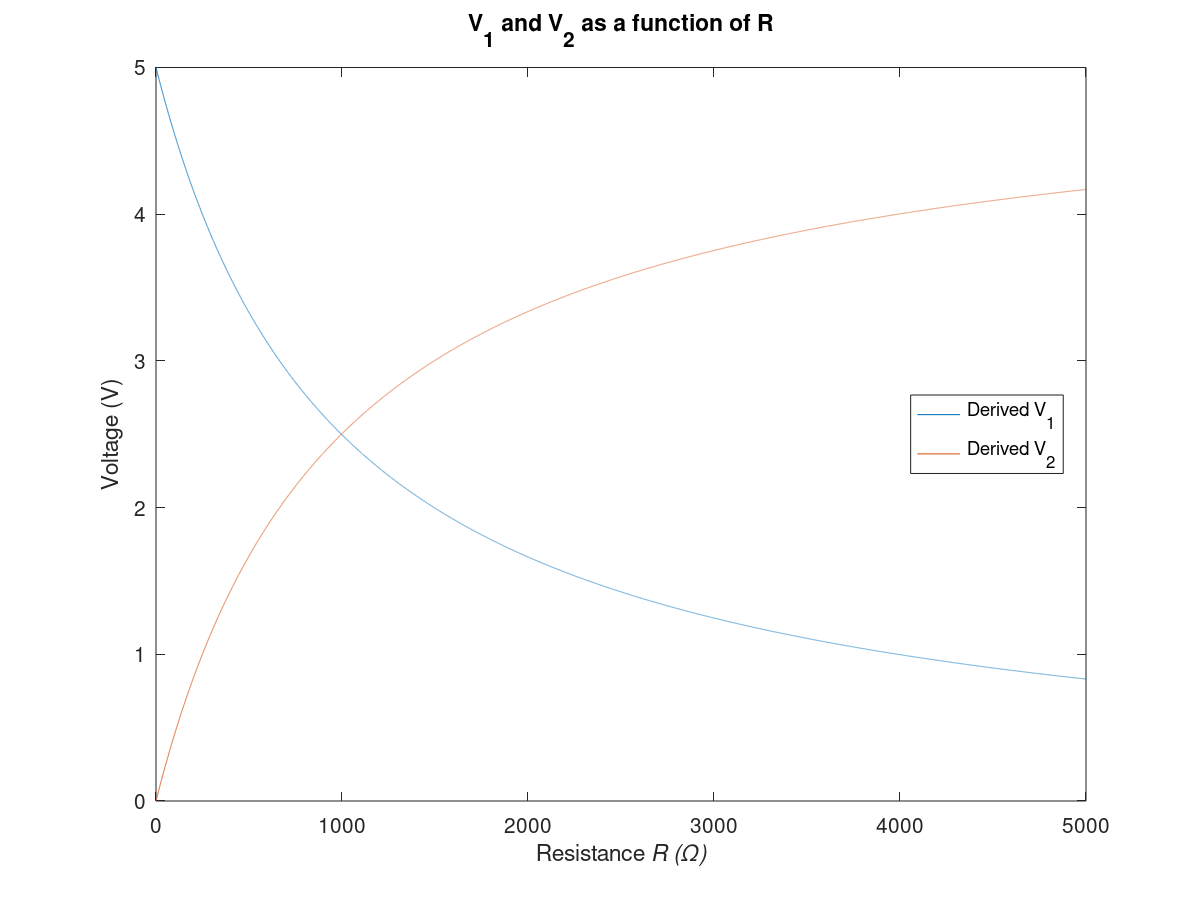
\includegraphics[width = 345pt]{chart.png}
\end{figure}

%3c
\subsection{Voltage $V_1$ and $V_2$ was measured as resistance R was changed}
Below is the data set obtained.
\begin{center}
    \begin{tabular}{S[table-format=4.1] S[table-format=1.3] S[table-format=1.6]}
        \toprule
        {R ($\Omega$)} & {$V_1$ (V)} & {$V_2$ (V)}\\
        \midrule
        1.6 & 4.98 & 0.000210 \\
        78 & 4.62 & 0.354 \\
        255 & 3.97 & 1.017 \\
        653 & 3.01 & 1.975 \\
        1101 & 2.37 & 2.61 \\
        1672 & 1.865 & 3.12 \\
        2050 & 1.633 & 3.35 \\
        2940 & 1.262 & 3.72 \\
        3500 & 1.107 & 3.88 \\
        4670 & 0.879 & 4.10 \\
        5000 & 0.830 & 4.15 \\ 
        \bottomrule
    \end{tabular}
\end{center}

\pagebreak

%3d
\subsection{A graph is generated using the above data set}
The data points were added to the previous graph illustrating its resemblance to the derived function.
\begin{figure}[H]
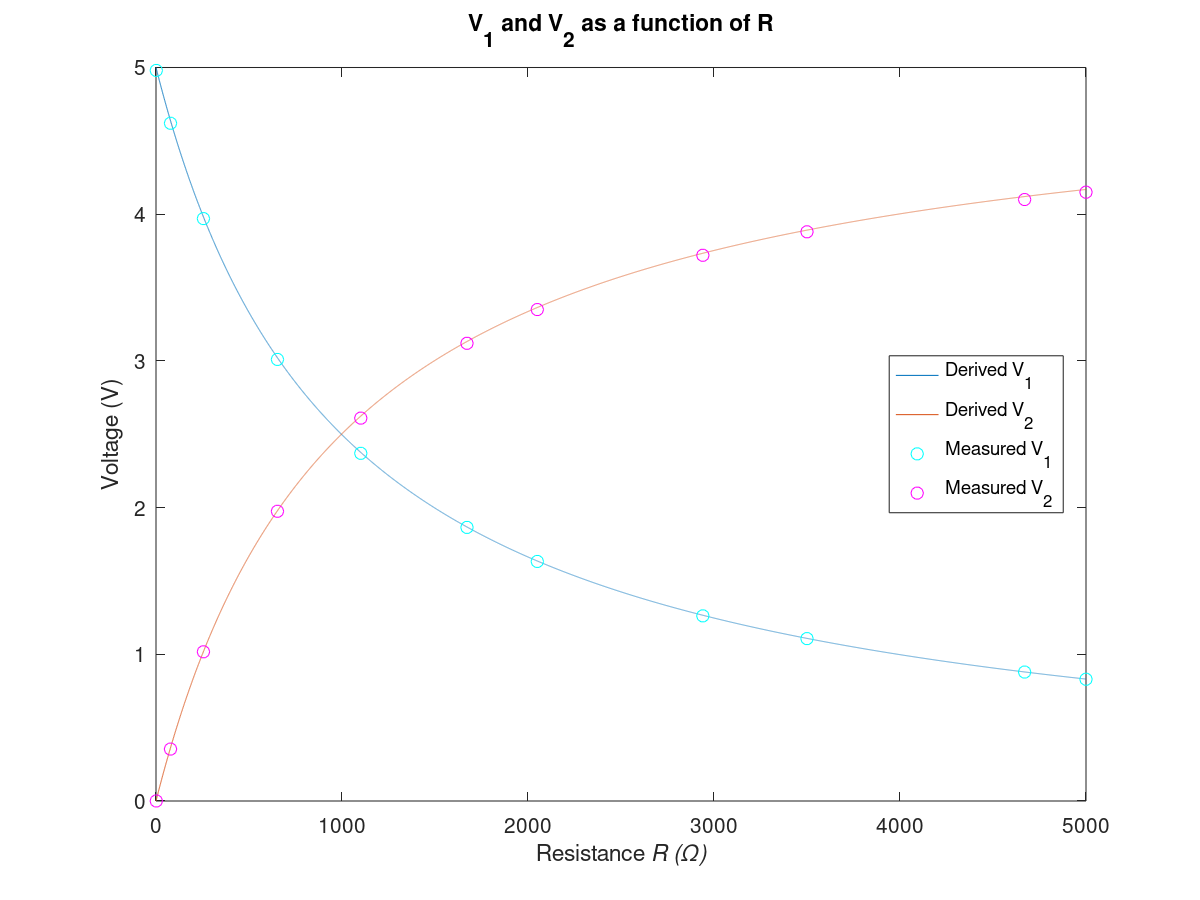
\includegraphics[width = 345pt]{chart2.png}
\end{figure}

%3e
\subsection{The data matched fairly closely with the derived equation}

\pagebreak

%4
\section{A circuit as illustrated below was set up with a \SI{5.00}{\volt} voltage source}
\begin{center}
    \begin{circuitikz}
        \draw 
            (2,2) 
            to[V_=$\SI{5}{\volt}$] (2,0)
            (2,2) --
            (3,2)to[R=$\SI{993}{\ohm}\approx\SI{1}{\kilo\ohm}$] 
            (5,2) --
            (6,2) to[R,l_=$\SI{991}{\ohm}\approx\SI{1}{\kilo\ohm}$,v^=$V_2$] (6,0)
            (6,2) -- 
            (9,2)to[R,l_=$R_M$] (9,0)--(2,0)
            ;
    \end{circuitikz}
\end{center}

%4a
\subsection{$V_2$ was measured in the original circuit i.e. when $R_M$ was detached}
In the original circuit, $V_2$ was measured to be \SI{2.48}{\volt}.

%4b
\subsection{$V_2$ would be relatively small if $R_M$ is relatively small}
\begin{align}
    \intertext{Let the equivalent resistance of the parallel configuration of \SI{991}{\ohm} resistor and $R_M$ be $R_{eq}$:}
    R_{eq} &= \frac{1}{\frac{1}{991}+\frac{1}{R_M}}
    \intertext{Let the equivalent resistance of the entire circuit be $R_t$:}
    R_t &= \SI{993}{\ohm}+R_{eq}
    \intertext{From voltage divider rule:}
    V_2 &= \frac{R_{eq}}{\SI{993}{\ohm}+R_{eq}} \cdot (\SI{5}{\volt})\\
\end{align}
If $R_M$ is relatively small, $\frac{1}{R_M}$ would be relatively large as it is inversely proportional to $R_M$; $R_{eq}$ would be relatively small as it is inversely proportional to $\frac{1}{R_M}$; $V_2$ would be relatively small as well as it is directly proportional to $R_{eq}$.

%4c
\subsection{A relatively small resistor $R_M$ was connected, and $V_2$ was measured to be relatively small}
A relatively small resistor with resistance of \SI{11.4}{\ohm} was connected as $R_M$, and $V_2$ was subsequently measured to be \SI{0.053}{\volt}, a value much smaller than the original value of $V_2$, \SI{2.48}{\volt}, as explained in part (b).

%4d
\subsection{A relatively large resistor $R_M$ was connected, and $V_2$ was measured to be the same as the original value}
A relatively large resistor with resistance of \SI{0.986}{\mega\ohm} was connected as $R_M$, and $V_2$ was subsequently measured to be \SI{2.48}{\volt}, the same as the original value of $V_2$, \SI{2.48}{\volt}.

%4e
\subsection{An ideal voltmeter should have a large equivalent resistance}
As demonstrated above, when a voltmeter with a small equivalent resistance was connected to the element measured, the measured value is far less than the actual value. Therefore, an ideal voltmeter should have a larger equivalent resistance.

\pagebreak

%5
\section{A circuit as illustrated below was set up with a \SI{6.00}{\volt} voltage source}
\begin{center}
    \begin{circuitikz}
        \draw 
            (0,2) 
            to[V_=$V_s\equal\SI{5}{\volt}$] (0,0)
            (0,2) to[short,i>^=$I_M$] 
            (1,2) to[R=$R_M$] (3,2)
            to[R=$\SI{993}{\ohm}\approx\SI{1}{\kilo\ohm}$] 
            (5,2) to[R,l_=$\SI{991}{\ohm}\approx\SI{1}{\kilo\ohm}$] (5,0)--(0,0)
            ;
    \end{circuitikz}
\end{center}

%5a
\subsection{$I_1$ was measured in the original circuit i.e. when $R_M$ was detached}
In the original circuit, $I_1$ was measured to be \SI{2.49}{\milli\ampere}.

%5b
\subsection{$I_M$ would be closer to original value, $I_1$, if $R_M$ is relatively small}
\begin{align}
    \intertext{Let the equivalent resistance of the entire circuit be $R_t$:}
    R_t &= \SI{993}{\ohm}+\SI{991}{\ohm}+R_t
    \intertext{From the Ohm's Law:}
    I_M &= \frac{V_s}{R_t} = \frac{5}{\SI{993}{\ohm}+\SI{991}{\ohm}+R_t}
\end{align}
If $R_M$ is relatively small, the equivalent resistance of the entire circuit would be closer to the original circuit and, as a result, $I_M$ would be closer to the original value.

%5c
\subsection{A relatively small resistor $R_M$ was connected, and $I_M$ was measured to be close to the original value}
A relatively small resistor with resistance of \SI{11.4}{\ohm} was connected as $R_M$, and $I_M$ was subsequently measured to be \SI{2.47}{\milli\ampere}, a value close to the original value of $I_1$, \SI{2.49}{\milli\ampere}, as explained in part (b).

%5d
\subsection{A relatively large resistor $R_M$ was connected, and $I_1$ was measured to be much smaller than the original value}
A relatively large resistor with resistance of \SI{0.986}{\mega\ohm} was connected as $R_M$, and $I_M$ was subsequently measured to be \SI{5}{\micro\ampere}, a value much smaller than the original value of $I_1$, \SI{2.49}{\milli\ampere}.

%5e
\subsection{An ideal voltmeter should have a small equivalent resistance}
As demonstrated above, when a voltmeter with a small equivalent resistance was connected to the element measured, the measured value is closer to the actual value. Therefore, an ideal voltmeter should have a small equivalent resistance.
\end{document}